\section{Security Model}

The BiobankCloud environment deploys strong security features for concerns such as confidentiality, integrity and non-repudiation~\cite{BBCSEC} of data access. This includes authentication, authorization, and auditing. The system allows defining different roles with different access privileges. In designing the system, we applied the Cloud Privacy Threat Modeling~\cite {CPTM} approach to identify the privacy requirements of processing sensitive biomedical data. This model implements a data management policy that aligns with the European data protection directive. The project further implements tools to ensure the correct allocation of legal responsibilities for the data processed within the platform. 

Figure \ref{fig:security} shows the different components of the employed security mechanisms. All BiobankCloud services are protected behind the firewall and only accessible through the secure interfaces over HTTPS channels.

%\vskip-5pt
\begin{figure}[h]
\centering
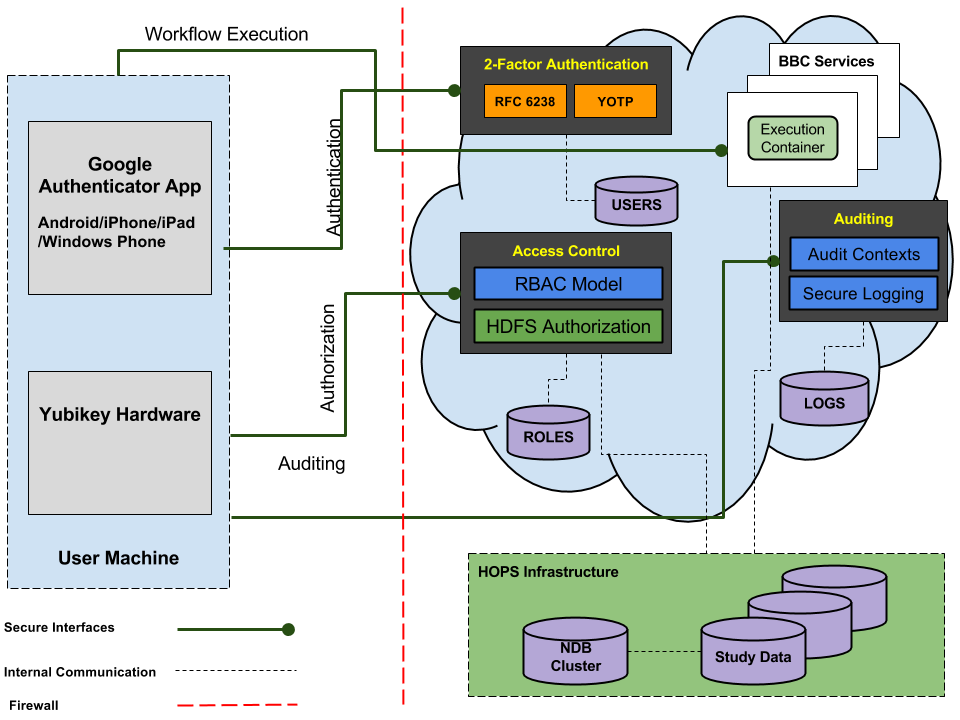
\includegraphics[width=0.8\textwidth]{./imgs/security.png}
\caption{Secure access to the BiobankCloud via a web front-end.}
\label{fig:security}
\end{figure}
%\vskip-5pt

\subsection{2-Factor Authentication}
The authentication services map the person accessing the platform to a user identity. We provide 2-factor authentication using smart mobile devices or Yubikey\footnote{Yubikey Manual, \url{http://www.yubico.com}} hardware tokens to support different groups of users. Users send authentication requests via a Web browser to the authentication service that runs instances of the time-based one-time password (TOTP) and Yubikey one-time password (YOTP) protocols.

In a mobile scenario, a user supplies an one-time generated password by a commercial authenticator in addition to a simple password that was decided during the account registration. The login page authenticates the user to the platform using the TOTP module (Time-Based One-Time Password) as an implementation of the RFC 6238.  In contrast, a Yubikey user would enter the Yubikey device into a USB port. The user enters the simple password that was decided during the account registration and pushes the Yubikey button. The Yubikey login page authenticates the user to the platform via the YOTP module.

\subsection {Role-based Access Control}

The access control component ensures authorized access to all data and services within a platform installation. file system level. Therefore, the system defines several roles\footnote{The concrete roles should be seen as implementations of the European Data Protection Directive.} which are granted certain access rights to certain studies. Examples are a DataOwner (users who may create new data sets), a DataScientist (users who can run workflows on the data), or an auditor (users with access to audit trails for auditing). DataSets technically can be shared between studies, and users may have different roles in different studies. We use the access control mechanism of HopsFS to implement the Study- and DataSet-based authorization model. 

\subsection {Auditing Service}
Finally, the auditing service enables the platform administrator or an external auditor to discover the history of accessing the platform to detect any violation to a policy. It includes several contexts such as role, account, study, and login audits. The secure login service assures that actions that are taken by the users are registered for tracing and auditing purposes. Each log event contains information such as initiator, target, IP/MAC addresses, timestamp, action, and outcome.
